\section{实证结果：边际效应}
\label{sec:marginal}

按定理 \ref{thm:threshold}，门控的相对优势是互补性、估计噪声与交易成本的函数。
本节对四个可操作的设计维度——交易成本、制度状态数、训练窗长度与横截面宽度——
估计边际效应。估计沿用主实验的滚动协议，在年份固定效应下计算斜率，
并以测试年份为聚类单位做 2\,000 次自助重抽样。

\begin{table}[htbp]
\centering
\caption{交易成本对门控相对优势的边际效应}
\label{tab:cost}
\begin{threeparttable}
\footnotesize
\begin{tabular}{lrrrr}
\toprule
单边成本 $\kappa$（基点） & 门控夏普 & 等权夏普 & 夏普差值 & 门控换手率 \\
\midrule
0 & 0.701 & 0.566 & $+0.135$ & 0.372 \\
5 & 0.690 & 0.562 & $+0.128$ & 0.372 \\
10 & 0.678 & 0.558 & $+0.120$ & 0.372 \\
20 & 0.656 & 0.550 & $+0.105$ & 0.372 \\
30 & 0.633 & 0.542 & $+0.091$ & 0.372 \\
50 & 0.588 & 0.526 & $+0.062$ & 0.372 \\
\midrule
\multicolumn{5}{l}{斜率（年份固定效应，年份聚类自助）：
$-0.001\,47$/基点，95\% 区间 $[-0.001\,72,-0.001\,21]$，$p<0.001$} \\
\multicolumn{5}{l}{每 10 个基点的边际效应：$-0.0147$；盈亏平衡成本（线性外推）：
约 92 个基点} \\
\bottomrule
\end{tabular}
\begin{tablenotes}[flushleft]\footnotesize
\item 注：数值为 12 个测试年份、3 个随机种子的均值（$N=216$）。
门控换手率（0.372）约为等权（0.131）的 2.8 倍，成本上升对门控的边际影响更大。
本表为与主实验同一协议的独立重跑，10 个基点处的基线差值为 $+0.120$，
与主实验的 $+0.115$ 相差 0.005，差异来自随机种子下训练过程的数值波动。
\end{tablenotes}
\end{threeparttable}
\end{table}

交易成本由 0 上升至 50 个基点，门控相对等权的夏普差值由 $+0.135$ 单调下降至
$+0.062$，降幅 54\%；斜率估计为每基点 $-0.001\,47$（$p<0.001$）。
每 10 个基点的成本上升使相对优势下降约 0.015。成本以
$2\lambda\kappa\mathcal{C}(\hat g)$ 的形式进入阈值，换手越高门槛越高，
实证方向与比较静态 H3 一致。线性外推显示相对优势在单边成本约 92 个基点时消失。
A 股主动权益基金的显性费率与隐性冲击成本之和通常低于这一水平，
高频调仓的小市值策略则可能接近该临界值。

零成本假设提供了另一条信息。即使 $\kappa=0$，门控相对等权的夏普差值也仅为 $+0.135$。
门控的表现限制不在交易成本：若限制来自成本项，降低换手即可改善；
而本文的阈值检验（$p=0.060$ 与 $0.065$）显示限制来自 $\hat\Gamma<\Theta$，
调整换手无法改变这一判断。

\begin{table}[htbp]
\centering
\caption{制度状态数的边际效应}
\label{tab:states}
\begin{threeparttable}
\footnotesize
\begin{tabular}{lrrrr}
\toprule
制度状态数 $S$ & 门控夏普 & 夏普差值 & 分段边际效应 & 理论净价值 $\Delta(S)$ \\
\midrule
2 & 0.602 & $+0.044$ & —— & $-9.23\times10^{-4}$ \\
3 & 0.682 & $+0.123$ & $S{:}\,2\to3$：$+0.079$ & $-1.02\times10^{-3}$ \\
4 & 0.668 & $+0.110$ & $S{:}\,3\to4$：$-0.014$ & $-1.11\times10^{-3}$ \\
\midrule
\multicolumn{5}{l}{线性斜率（年份固定效应）：$+0.032\,8$/状态，95\% 区间
$[0.000\,4,0.066\,1]$，$p=0.047$} \\
\bottomrule
\end{tabular}
\begin{tablenotes}[flushleft]\footnotesize
\item 注：状态按 12 个月市场收益的分位数划分，并以 one-hot 形式并入门控输入。
夏普为 12 个测试年份、2 个随机种子的平均（$N=72$）。
理论净价值按式 \eqref{eq:delta-S} 计算（$\lambda=5$，门控参数 200 个）；
其绝对水平受容量项量级影响，此处关注其随 $S$ 的变化方向。
线性斜率包含 $S=2$ 到 $S=3$ 的跃升，掩盖了转折点，分段边际效应更能反映内点最优。
\end{tablenotes}
\end{threeparttable}
\end{table}

门控表现在 $S=3$ 处达到最高（0.682），$S=2$ 时为 0.602，$S=4$ 时回落至 0.668，
呈内点最优。分段边际效应为 $2\to3$ 提升 0.079、$3\to4$ 下降 0.014，
边际收益在 $S=3$ 处转负。制度数增加提高可用互补性 $\Gamma(S)$，
同时提高估计误差成本 $\Theta(S)$ 与容量成本；当后者的边际成本超过前者的边际收益时，
净价值开始下降（定理 \ref{thm:optimal-S}）。

理论净价值与实证最优点存在定量差异。按式 \eqref{eq:delta-S} 使用名义门控参数量
（200 个）计算，净价值在所有 $S$ 下均为负，最优点落在 $S=2$，
容量项 $\sigma^2d_{\text{gate}}/T$ 以 $200/247$ 的量级主导了净价值。
该差异印证定理 \ref{thm:optimal-S} 的核心含义：在 $T=247$ 的样本量下，
200 个自由参数的门控处于容量约束的紧边界上。实证中最优的 $S=3$ 由验证窗在
$3\times2$ 网格中选出，其有效自由度远低于名义值。内点最优的方向得到支持，
精确定位需要更大样本或更小容量的门控架构。

\begin{table}[htbp]
\centering
\caption{训练窗长度的边际效应}
\label{tab:trainlen}
\begin{threeparttable}
\small
\begin{tabular}{lrrr}
\toprule
训练窗长度 & 窗口数 & 门控夏普 & 相对等权夏普差值 \\
\midrule
3 年 & 36 & 0.727 & $+0.213$ \\
5 年 & 36 & 0.678 & $+0.120$ \\
8 年 & 33 & 0.703 & $+0.163$ \\
\midrule
\multicolumn{4}{l}{线性斜率（年份固定效应）：$-0.006\,3$/年，
95\% 区间 $[-0.030\,8,0.018\,3]$，$p=0.617$} \\
\bottomrule
\end{tabular}
\begin{tablenotes}[flushleft]\footnotesize
\item 注：训练窗缩短减少门控的可用样本（提高 $\Theta$），
同时使训练数据更接近当前市场结构（降低结构变化带来的设定误差）。
样本窗口数因可用历史长度而异（$N=105$）。
\end{tablenotes}
\end{threeparttable}
\end{table}

训练窗长度。表 \ref{tab:trainlen} 不支持比较静态 H4 的简单形式。3 年训练窗的相对优势最高
（$+0.213$），8 年次之（$+0.163$），5 年最低（$+0.120$），呈非单调模式，
线性斜率的 95\% 区间跨越零。估计误差机制（$\Theta\propto1/T$）与结构变化机制
在此方向相反：更长的训练窗降低抽样误差，同时引入更多来自不同市场结构的陈旧信息，
提高设定误差。A 股在 2014--2026 年间经历注册制改革、涨跌停制度调整与投资者结构变化，
信号有效性随时间漂移，结构变化的力量在本样本中占优，最优训练窗长度约为 3 年。

该结果指向一个更一般的判断：定理 \ref{thm:threshold} 中的 $T$ 应理解为
来自同一数据生成过程的有效样本量，而非日历长度。
在结构变化明显的市场上，延长训练窗不必然降低 $\Theta$。
以「训练样本更长」为由扩大模型容量，在市场结构快速变化的环境下未必成立。

横截面宽度。横截面宽度与上述三个维度不同：它不可由研究者调节，却决定机制能否被识别。
两条渠道的噪声底线按不同速率收敛，$\Theta^{(1)}\asymp c_1(S-1)/T$，
$\Theta^{(2)}\asymp c_2(S-1)/(NT)$；互补性统计量的上界以 $1/N$ 收缩。
在宽横截面上，二阶渠道的噪声底线以 $1/N$ 的速率下降，识别能力显著改善；
扩大横截面对一阶渠道不带来识别增益。

本文的两个样本给出直接对照。A 股样本的平均横截面宽度约为 438 只，
互补性统计量处于阈值边缘（$p=0.060$ 与 $0.065$）；十只美国 ETF 的样本上，
月度横截面回归因每月证券数不足 20 只而无法估计，互补性检验不可识别。
后者的原因不是实现质量，而是 $\hat\Gamma$ 的上界因 $N=10$ 而低于噪声底线。
以少数 ETF 为样本、却报告多智能体门控优势的研究，在本文框架下面临这一识别问题。

\begin{figure}[htbp]
\centering
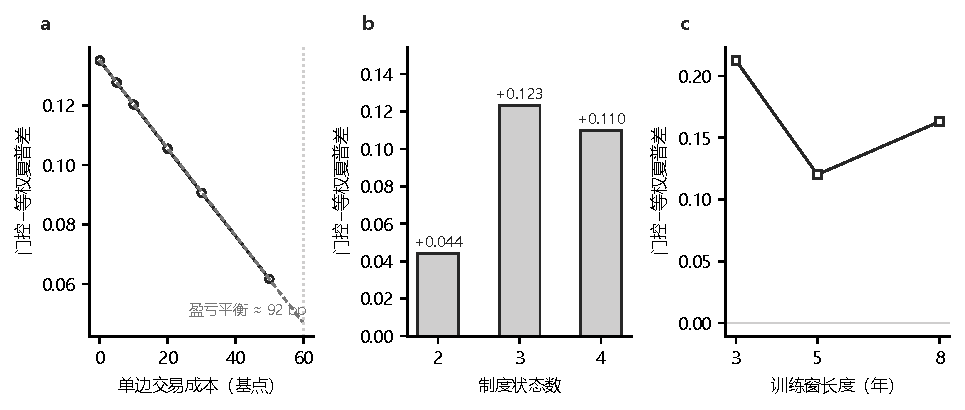
\includegraphics[width=\textwidth]{fig_marginal.pdf}
\caption{三个设计维度的边际效应}
\label{fig:marginal}
\begin{minipage}{0.94\textwidth}\footnotesize
注：(a) 交易成本：散点为各成本水平的夏普差值均值，虚线为年份固定效应下的线性拟合，
点线标出线性外推的盈亏平衡成本（约 92 个基点）；
(b) 制度状态数：由 2 增至 3 提升 0.079，由 3 增至 4 下降 0.014；
(c) 训练窗长度：3 年、5 年、8 年分别为 $+0.213$、$+0.120$、$+0.163$，非单调。
\end{minipage}
\end{figure}

\begin{table}[htbp]
\centering
\caption{边际效应估计汇总}
\label{tab:marginal-sum}
\begin{threeparttable}
\footnotesize
\begin{tabular}{lp{3.6cm}rrp{3.2cm}}
\toprule
维度 & 边际效应 & 95\% 区间 & $p$ 值 & 对应的理论含义 \\
\midrule
交易成本 & $-0.001\,47$/基点 & $[-0.001\,72,-0.001\,21]$ & $<0.001$ & H3：成本线性进入阈值 \\
\quad（换算） & $-0.0147$/10 基点 & —— & —— & 盈亏平衡约 92 基点 \\
制度状态数 & $+0.032\,8$/状态 & $[0.000\,4,0.066\,1]$ & 0.047 & H1：净价值单峰 \\
\quad（分段） & $2\to3$：$+0.079$；$3\to4$：$-0.014$ & —— & —— & 内点最优在 $S=3$ \\
训练窗长度 & $-0.006\,3$/年 & $[-0.030\,8,0.018\,3]$ & 0.617 & H4：不支持简单形式 \\
横截面宽度 & 不可调节 & —— & —— & 一阶 $\Theta\propto1/T$，二阶 $\Theta\propto1/(NT)$ \\
持续性乘数 & 放大 19.5 倍 & —— & —— & H5：$\mathcal{M}=(I-\beta P)^{-1}$ \\
\bottomrule
\end{tabular}
\begin{tablenotes}[flushleft]\footnotesize
\item 注：斜率均在年份固定效应下估计，以测试年份为聚类单位做 2\,000 次自助重抽样；
$p$ 值为对零的双侧自助检验。交易成本面板 $N=216$，制度数面板 $N=72$，
训练窗面板 $N=105$，均为测试年份与随机种子的组合。
\end{tablenotes}
\end{threeparttable}
\end{table}

四个维度的估计给出一个统一判断：门控的净价值对交易成本高度敏感，
对制度数呈内点最优，对训练窗长度不敏感。提高模型复杂度的边际回报很小甚至为负，
控制换手与成本、把制度数控制在样本量容许的范围内，才是提高净价值的关键。
